%!TEX root =  ..\ekg_7_projektbericht.tex

%PCB Design

\subsection{Platinendesign}

Für das zeichnen von Schaltplänen sowie dem Layouten des PCBs wird das Programm Altium Designer verwendet. Es beinhaltet eine übersichtliche Benutzeroberfläche und zahlreiche Features wie PCB-Design in nativem 3D, interaktives Routing, hierarchische Designs, einheitliche Bibliothekenverwaltung, integrierte SPICE Simulationen und zahlreiche Export-Möglichkeiten in einem Tool. 

%TODO Abkürzungen ins Abkürzungsverzeichnis schreiben

\subsubsection{Erstellung von Libraries}
Da in der integrierten Datenbank von Altium Designer nicht alle benötigten Bauteile enthalten sind, müssen diese zunächst von Hand angelegt werden. Dieser Prozess gliedert sich in drei Schritte:

\begin{enumerate}
\item Erstellung des Schaltzeichens:\\
Hierbei wird mithilfe von geometrischen Formen ein Symbol des Bauteils erstellt, welches möglichst gut seine Funktion widerspiegelt. Idealerweise dient dafür ein Symbol des Herstellers als Vorlage, welches nachgestellt werden kann. Hierbei müssen bereits die Ein- und Ausgangspins des Bauteils festgelegt werden, da nur dort später Leitungen angeschlossen werden können. Den Pins wird eine Nummer zugewiesen, welche später einem Pad des Footprints entspricht.

\item Erstellung des Footprints: \\
Für jeden Pin des Bauteils muss ein Pad auf dem PCB erstellt werden, auf welchem das Beinchen später aufliegt und verlötet wird. Dabei ist auf eine Ausreichende Größe des Pads zu achten, damit das Beinchen vollständig verbunden werden kann. Es empfiehlt sich, die Pads länger als nötig zu gestalten, wenn im Nachgang noch Bauteile per Hand verlötet werden sollen. Idealerweise verwendet das Bauteil einen Standard-Footprint, welchen es bereits als Vorlage gibt. 

\item Hinzufügen eines 3D Modells: \\
Um die Platine später in 3D zu bearbeiten und vollständig zu exportieren werden jedem Bauteil dreidimensionale Modelle hinzugefügt. Dies ist in Altium durch den import einer .step Datei möglich. Diese muss im Anschluss noch genau auf das Pad ausgerichtet werden.
\end{enumerate}

\subsubsection{Zeichnen des Schaltplans}
Der Schaltplan wird auf Basis vorhergegangener Versuche durchgeführt. Sobald eine Baugruppe erfolgreich getestet ist, wird sie in den Schaltplan integriert. Vor dem Anlegen der einzelnen Seiten wird ein Template erstellt, was eine einheitliche Form des Schaltplans gewährleistet und Informationen wie Projektname, Ersteller, Revisionsnummer, etc. vermittelt. Der Schaltplan ist auf vier Seite aufgeteilt:

\begin{enumerate}
\item Power Supply
\item MCU
\item Filterung
\item Peripherie
\end{enumerate}

Die Nummerierung von Seiten und Bauteilen wurde so konfiguriert, dass diese automatische durch Altium erfolgt. Der Schaltplan ist in funktionale Blöcke untergliedert, welche mit einem kurzen Kommentar beschriftet sind. Dies erleichtert die Übersichtlichkeit (Abbildung \ref{fig:sch_ps}).

\begin{figure} [!h]
	%\centering
	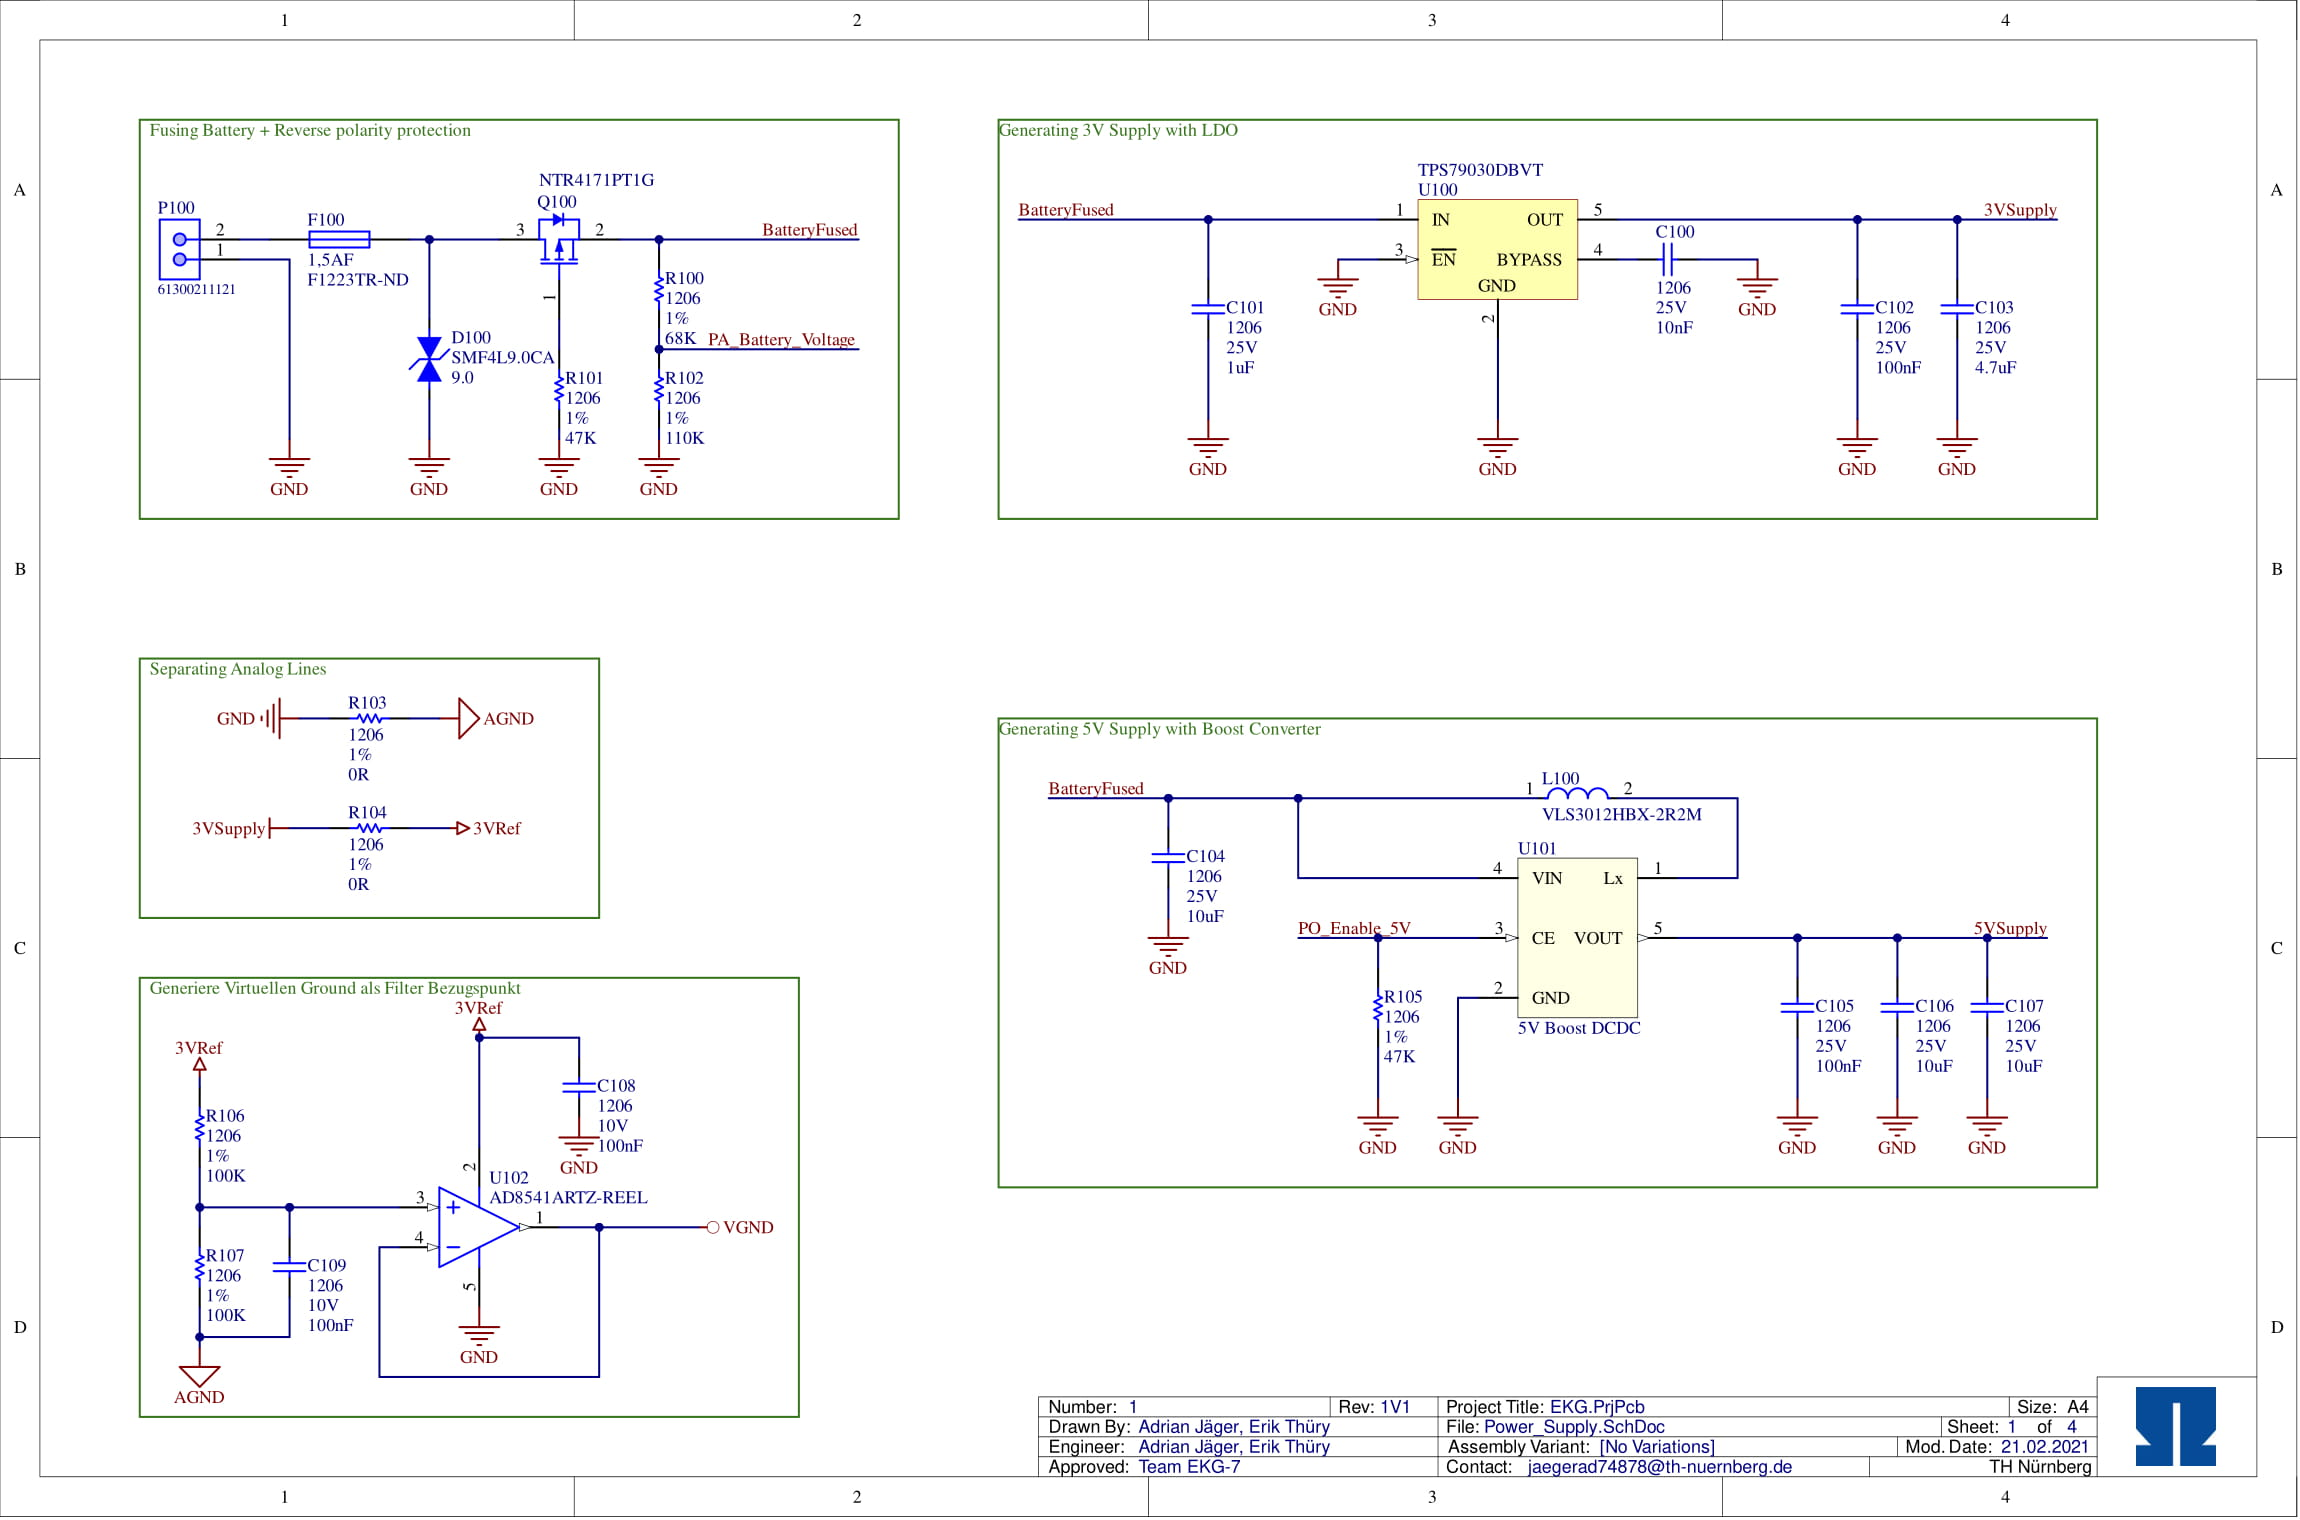
\includegraphics[width=\textwidth] {Schematics_EKG_2021-02-21_Power_Supply}
	\caption{Schaltplan Seite Power Supply}
	\label{fig:sch_ps} 
\end{figure}

Weiterhin werden Kondensatoren parallel zu den Versorgungspins sämtlicher ICs eingeplant. Dies verhindert, dass sich Schwankungen in der Versorgungsspannung auf den IC und Lastwechsel des ICs auf die Versorgungsspannung auswirken.

\subsubsection{Platzieren der Komponente}
Nach dem Abschluss des Schaltplans kann mit dem Layout der Platine begonnen werden. Hierfür wird zunächst in Absprache mit dem Gehäuseverantwortlichen eine Maximalgröße der Platine festgelegt. Die Abmaße werden im Board Planning Mode des neu erstelltem PCB Documents in Altium Designer eingetragen.

Für die Platzierung wird zunächst eine grobe Skizze auf Papier erstellt (Abbildung \ref{fig:p_layout} . Damit wird bereits jeder Baugruppe ein Raum auf der Platine zugesichert, von welchem aus alle Verbindungen zu anderen Baugruppen gut erreichbar sind. 

Die MCU rückt dabei in den Mittelpunkt, da von ihr aus Verbindungen zu allen Baugruppen bestehen. Bei ihr ist darauf zu achten, das sämtliche vom Hersteller geforderten Bypass-Kondensatoren so nah wie möglich an den entsprechenden Pins Platziert werden. Selbiges gilt für den externen Hochfrequenz-Schwingquarz, dessen Zuleitungen ebenfalls nur kurze Distanzen überbrücken sollte.

Die Absicherung der Spannungsversorgung ist in unmittelbarer nähe zum Anschluss an die Batterie zu platzieren. Der 3D Modus ist beim Platzieren von Bauteilen hilfreich um die Platzverhältnisse besser einzuschätzen.

\begin{figure} [!h]
	%\centering
	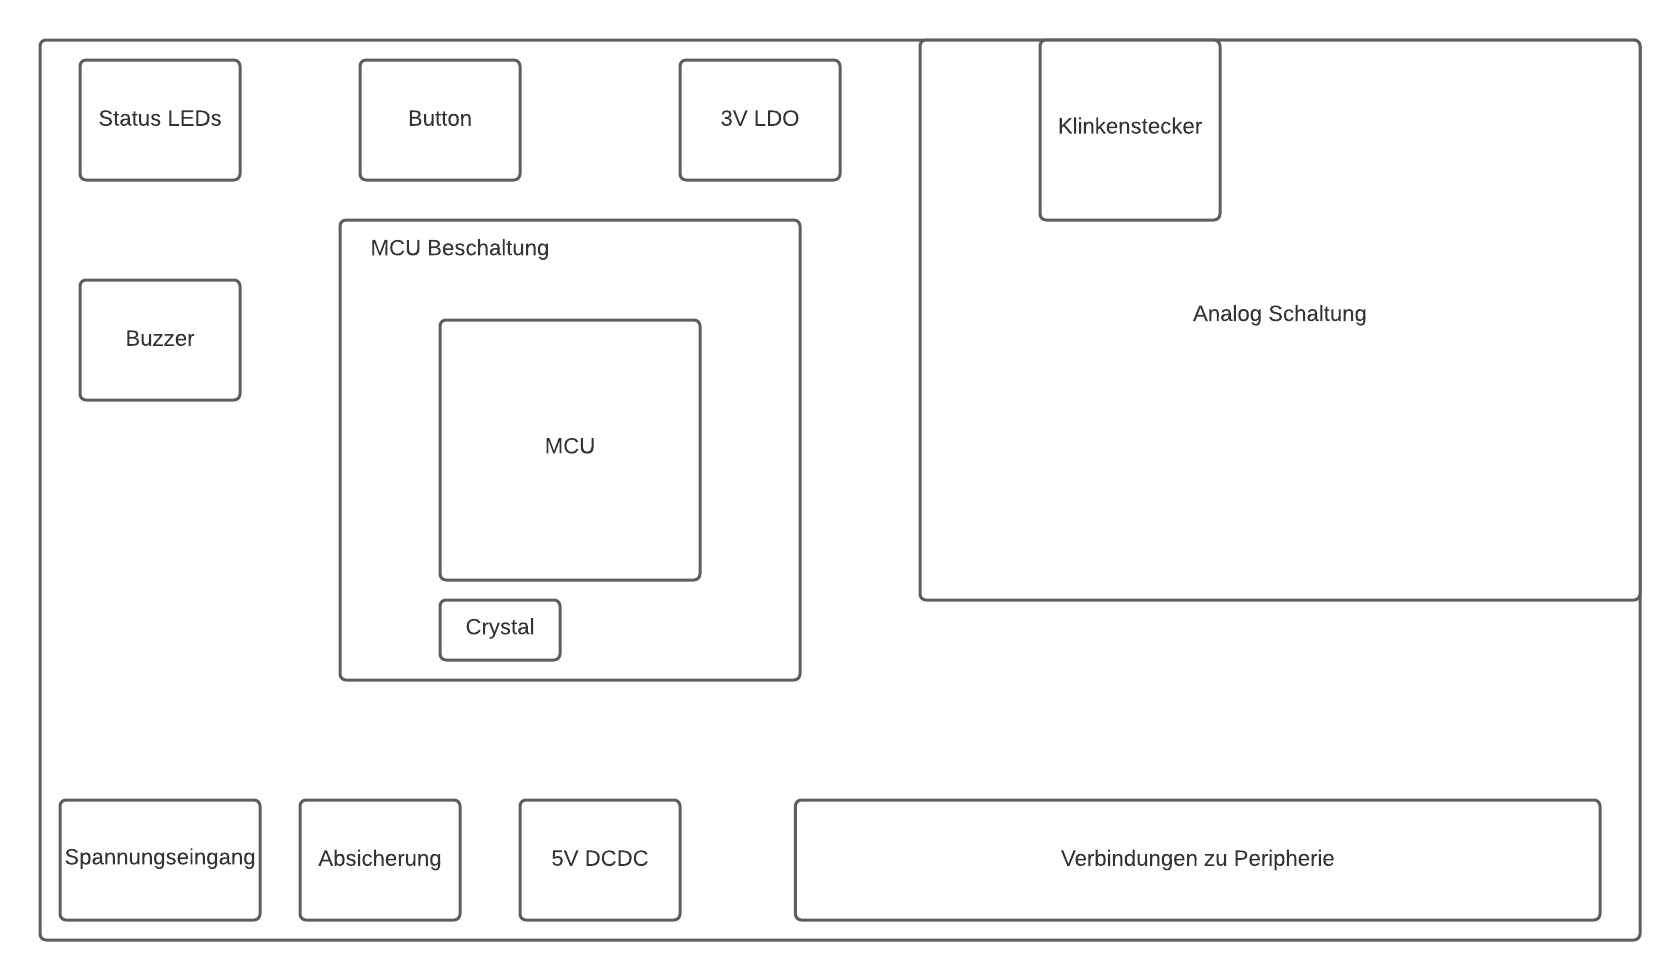
\includegraphics[width=\textwidth] {Platinenlayout_skizze}
	\caption{Skizze des Platinenlayouts}
	\label{fig:p_layout} 
\end{figure}


\subsubsection{Routing}



\subsubsection{Fertigung und Bestückung}

\subsubsection{Inbetriebnahme}